\documentclass[10pt]{article}

\usepackage[T1]{fontenc}
\usepackage{lmodern}
\usepackage[margin=0.78in]{geometry}
\usepackage{microtype}
\usepackage{amsmath,amssymb,amsthm,mathtools}
\usepackage{booktabs}
\usepackage{array}
\usepackage{enumitem}
\usepackage{xcolor}
\usepackage{tikz}
\usetikzlibrary{arrows.meta,positioning}
\usepackage[numbers,sort&compress]{natbib}
\usepackage[colorlinks=true,linkcolor=blue!55!black,citecolor=blue!55!black,urlcolor=blue!55!black]{hyperref}
\hypersetup{
  pdftitle={ZKSM83: Native Lookup Proofs for SM83 Execution},
  pdfauthor={Ryan Kung},
  pdfsubject={Native SM83 lookup arguments and transparent lattice-backed receipts},
  pdfkeywords={SM83, zkVM, sumcheck, lookup argument, Akita, Module-SIS}
}

\setlength{\parindent}{0pt}
\setlength{\parskip}{3pt}
\setlist{nosep,leftmargin=1.4em}
\allowdisplaybreaks
\numberwithin{equation}{section}

\definecolor{ink}{HTML}{17212B}
\definecolor{accent}{HTML}{375A7F}
\definecolor{soft}{HTML}{EEF3F7}
\color{ink}

\newcommand{\F}{\mathbb{F}}
\newcommand{\B}{\{0,1\}}
\newcommand{\Com}{\mathsf{Com}}
\newcommand{\Open}{\mathsf{Open}}
\newcommand{\Verify}{\mathsf{Verify}}
\newcommand{\Enc}{\mathsf{Enc}}
\newcommand{\Hash}{\mathsf{H}}
\newcommand{\eq}{\operatorname{eq}}
\newcommand{\mle}{\widetilde}
\newcommand{\Stmt}{\mathsf{Stmt}}
\newcommand{\Trace}{\mathsf{Trace}}
\newcommand{\Rel}{\mathcal{R}}
\newcommand{\Lang}{\mathcal{L}}
\newcommand{\one}{\mathbf{1}}
\newcommand{\zero}{\mathbf{0}}
\newcommand{\code}[1]{\texttt{#1}}
\newcommand{\ok}{\ensuremath{\checkmark}}
\newcommand{\unknown}{\ensuremath{?}}
\DeclareMathOperator{\MSIS}{MSIS}
\DeclareMathOperator{\poly}{poly}
\DeclareMathOperator{\negl}{negl}

\newtheorem{proposition}{Proposition}
\newtheorem{definition}{Definition}

\title{\vspace{-1.6em}\textbf{ZKSM83: Native Lookup Proofs for SM83 Execution}\\
\large Transparent lattice-backed receipts for the DMG/MBC3 machine}
\author{Ryan Kung}
\date{Implementation snapshot \code{1062c35} \;\textperiodcentered\; September 2026}

\begin{document}
\maketitle
\vspace{-1.3em}

\begin{abstract}
ZKSM83 proves CPU-visible execution of an SM83 machine directly.  A segment packs at most four
instructions per row into $N=2^{14}$ rows, commits $C=4604$ multilinear columns, and checks
$M=11458$ identities of degree at most $23$ by sumcheck and a transparent Akita polynomial
commitment scheme.  ISA, byte-operation, ROM, memory, device, log, and segment-boundary claims
share one committed trace.  Version 2 is transparent, not witness-hiding; no current end-to-end
packed-proof measurement is claimed.
\end{abstract}

\begin{center}
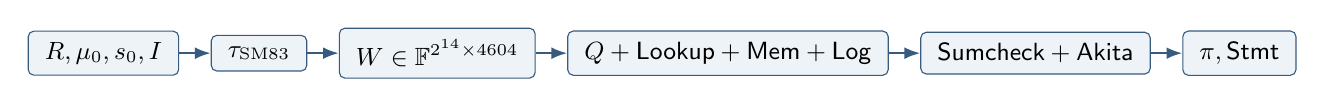
\begin{tikzpicture}[
  node distance=4mm,
  box/.style={draw=accent,rounded corners=2pt,fill=soft,inner xsep=6pt,inner ysep=4pt,font=\small},
  arr/.style={-{Latex[length=2mm]},thick,draw=accent}
]
\node[box] (in) {$R,\mu_0,s_0,I$};
\node[box,right=of in] (tau) {$\tau_{\rm SM83}$};
\node[box,right=of tau] (w) {$W\in\F^{2^{14}\times4604}$};
\node[box,right=of w] (rel) {$Q+\mathsf{Lookup}+\mathsf{Mem}+\mathsf{Log}$};
\node[box,right=of rel] (pcs) {$\mathsf{Sumcheck}+\mathsf{Akita}$};
\node[box,right=of pcs] (out) {$\pi,\Stmt$};
\draw[arr] (in)--(tau);
\draw[arr] (tau)--(w);
\draw[arr] (w)--(rel);
\draw[arr] (rel)--(pcs);
\draw[arr] (pcs)--(out);
\end{tikzpicture}
\end{center}

\section{Proposition}

Let
\begin{equation}
 s_t=(x_t,d_t,m_t,c_t)\in
 \underbrace{\mathcal X_{\rm CPU\,+\,MBC3}}_{21\ \text{scalars}}
 \times\underbrace{\mathcal D_{\rm DMG}}_{17\ \text{scalars}}
 \times\mathcal M_{2^{17}}
 \times\mathbb N^4,
 \qquad |s_t|_{\rm public}=38.
\end{equation}
Here $c_t=(c_t^{\rm in},c_t^{\rm out},c_t^{\rm bus},c_t^{\rm isa})$ and
\begin{equation}
 (s_{t+1},\epsilon_t)=\tau_{R,I}(s_t),
 \qquad
 \epsilon_t=(\epsilon_t^{\rm bus},\epsilon_t^{\rm in},
              \epsilon_t^{\rm out},\epsilon_t^{\rm isa}).
\end{equation}

The public statement is
\begin{align}
 \Stmt={}&(\nu,D_{\rm back},p,|R|,C_R,B_0,B_L,L,T,A,C,\mathbf n), \\
 \mathbf n={}&(n_{\rm bus},n_{\rm in},n_{\rm out},n_{\rm isa}), \\
 \mathsf{id}(\Stmt)={}&\Hash(\code{zksm83/native-statement/v2}\parallel\Enc(\Stmt)),
 \label{eq:statement}
\end{align}
where $L,T,A,C$ are segment, source-transition, active-row, and machine-cycle counts.

\begin{definition}[Implemented language]
\begin{equation}
\Lang_{\rm SM83}=\left\{\Stmt:\exists\omega\quad
\Rel_{\rm row}(\omega)\wedge
\Rel_{\rm lookup}(\omega)\wedge
\Rel_{\rm mem}(\omega)\wedge
\Rel_{\rm log}(\omega)\wedge
\Rel_{\rm chain}(\omega,\Stmt)=1\right\}.
\end{equation}
\end{definition}

The semantic boundary is
\begin{align}
 \Rel_{\rm proved}={}&
 \{\text{SM83},\text{MBC3}_{\neg\rm RTC},\text{timer},\text{PPU timing/IRQ},
 \text{DMA},\text{serial},\text{joypad},\text{APU/MMIO}\},\\
 \Rel_{\rm excluded}={}&
 \{\text{pixels},\text{audio samples},\text{physical-chip provenance},
 \text{ROM ownership},\text{witness hiding}\}.
 \label{eq:scope}
\end{align}
The SM83 timing and opcode model follows the public hardware references in Pan Docs
\citep{pandocs,gbopcodes}; the proof architecture is lookup-centric in the sense of Jolt and Lasso
\citep{jolt,lasso}.

\section{Packed trace}

One segment uses the Boolean hypercube
\begin{equation}
 \mathcal H=\B^{14},\qquad N=|\mathcal H|=16384.
\end{equation}
For row $r\in\mathcal H$, let $a_r$ be active, $i_r$ be an instruction-block tag,
$\ell_{r,j}$ be lane activity, and $e_{r,k}$ be a machine-event selector:
\begin{align}
 a_r(a_r-1)&=i_r(i_r-1)=\ell_{r,j}(\ell_{r,j}-1)=e_{r,k}(e_{r,k}-1)=0,\\
 \ell_{r,0}&=i_r,
 &\ell_{r,j+1}(1-\ell_{r,j})&=0,\\
 a_r&=i_r+\sum_k e_{r,k},
 &i_r\sum_k e_{r,k}&=0,\\
 1\leq \sum_{j=0}^{3}\ell_{r,j}&\leq4 &&(i_r=1).
 \label{eq:row-tags}
\end{align}

Resource ownership is explicit.  For $S_M=6$ machine-cycle slots, $S_B=5$ bus slots,
and $\omega^{X}_{r,s,j}\in\B$:
\begin{align}
 \sum_{j=0}^{3}\omega^{X}_{r,s,j}&\in\B,
 &&X\in\{M,B\},\quad 0\le s<S_X,\\
 (1-\ell_{r,j})\sum_s\omega^{X}_{r,s,j}&=0,\\
 \ell_{r,j}\prod_{q=1}^{S_X}\left(\sum_s\omega^{X}_{r,s,j}-q\right)&=0.
 \label{eq:ownership}
\end{align}

The five local boundaries $x_{r,0},\ldots,x_{r,4}$ are shared across four lanes; the
device boundary $(d_r^-,d_r^+)$ is shared across the row:
\begin{align}
 \ell_{r,j}\bigl(x_{r,j+1}-\tau^{\rm cpu}_{o_{r,j}}(x_{r,j},b_{r,j})\bigr)&=0,\\
 (1-\ell_{r,j})(x_{r,j+1}-x_{r,j})&=0,\\
 e_{r,k}\bigl(d_r^+-\Delta_k(d_r^-,b_r,I_r)\bigr)&=0.
 \label{eq:lane-transition}
\end{align}

For lane $j$, local bus slot $u$, shared slot $s\ge u$, define $k=s-u$ and
\begin{align}
 f_{r,j,k}&=\omega^B_{r,k,j}
 \begin{cases}
 1,&k=0,\\
 1-\omega^B_{r,k-1,j},&k>0,
 \end{cases}\\
 m_{r,j,u,s}&=
 \begin{cases}
 f_{r,j,k},&u=0,\\
 f_{r,j,k}\,\omega^B_{r,s,j},&u>0,
 \end{cases}\\
 b_{r,j,u}&=\sum_{s=u}^{4}m_{r,j,u,s}b_{r,s}.
 \label{eq:bus-projection}
\end{align}
The $4\sum_{u=0}^{4}(5-u)=60$ values $m_{r,j,u,s}$ are committed columns.  This replaces
repeated cubic routing expressions by degree-one consumers.

The complete column geometry is
\begin{align}
 C&=3542+806+256=4604,\\
 806&=\underbrace{5\cdot106}_{\rm shared\ boundaries}
      +\underbrace{4\cdot54}_{\rm lane\ auxiliaries}
      +\underbrace{60}_{\rm bus\ matches},\\
 256&=\underbrace{4}_{\rm lanes}\cdot
      \underbrace{2}_{\rm execution\ queries}\cdot
      \underbrace{(1+19+12)}_{\rm selector+address+output}.
 \label{eq:columns}
\end{align}

\begin{table}[t]
\centering
\small
\begin{tabular}{@{}lrrr@{}}
\toprule
Relation prefix & columns & identities & degree \\
\midrule
Routing & 50 & 129 & 7 \\
Boundary & 145 & 297 & 3 \\
Front end & 729 & 1096 & 7 \\
Machine & 796 & 1353 & 7 \\
Mutable-memory row relation & 3542 & 8257 & 15 \\
Packed CPU plus execution lookup & 4604 & 11458 & 23 \\
\bottomrule
\end{tabular}
\caption{Source-asserted prefix geometry.  Prefix rows share columns; counts are not additive.}
\label{tab:geometry}
\end{table}

\section{Row relation}

Let $W_r\in\F^{4604}$.  The deepest relation is
\begin{align}
 Q(W_r)&=(Q_0(W_r),\ldots,Q_{11457}(W_r))=\zero,\\
 Q={}&Q_{\rm route}\cup Q_{\rm boundary}\cup Q_{\rm ISA}\cup Q_{\rm bus}
 \cup Q_{\rm flow}\cup Q_{\rm machine}\cup Q_{\rm device}\cup Q_{\rm MMIO}
 \cup Q_{\rm mem}\cup Q_{\rm CPU}\cup Q_{\rm exec-wf},\\
 \max_j\deg Q_j&\le23.
 \label{eq:deep-relation}
\end{align}

Byte and word reconstruction uses Boolean limbs:
\begin{align}
 b_k(b_k-1)&=0,&v&=\sum_{k=0}^{7}2^k b_k,\\
 w_k(w_k-1)&=0,&u&=\sum_{k=0}^{15}2^k w_k.
\end{align}
Typical selector-gated identities are
\begin{align}
 q_{\rm add}\,[r-a-b+2^8c]&=0,\\
 q_{\rm sub}\,[a-b-r-2^8c]&=0,\\
 q_{\rm jump}\,[pc^+-(q_t t+(1-q_t)pc_{\rm seq})]&=0,\\
 q_{\rm stack}\,[sp^+-(sp+\delta_{\rm sp})]&=0.
 \label{eq:cpu-families}
\end{align}
Flags, DAA, CB-prefixed operations, interrupts, HALT, MBC3 bank selection, timer stages,
PPU/STAT ordering, DMA, serial, joypad, APU, and typed MMIO instantiate the same pattern
$q\cdot f(W_r)=0$.

The fixed tables are
\begin{equation}
 T_{\rm ISA}:[2^9]\to\F^{38},\qquad
 T_{\rm exec}:[2^{19}]\to\F^{12},\qquad
 R:[2^{20}]\to\F.
 \label{eq:tables}
\end{equation}
There are four ISA queries, at most eight byte-operation queries, and at most five ROM bus
queries per packed row.

\section{Shout-style lookup equations}

For a table $T:\B^m\to\F^v$, selected trace rows $x\in\mathcal H$, address bits
$A(x)\in\B^m$, selector $q(x)$, and output $y(x)$, sample $\gamma,\lambda$ and compress
\begin{align}
 T_\gamma(u)&=\sum_{h=0}^{v-1}\gamma^hT_h(u),
 &y_\gamma(x)&=\sum_{h=0}^{v-1}\gamma^hy_h(x),\\
 \chi_{A(x)}(u)&=\prod_{j=0}^{m-1}
 \bigl(A_j(x)u_j+(1-A_j(x))(1-u_j)\bigr),\\
 R_A(u)&=\sum_{x\in\mathcal H}\lambda_xq(x)\chi_{A(x)}(u).
\end{align}
Then
\begin{equation}
 \boxed{
 \sum_{u\in\B^m}R_A(u)T_\gamma(u)
 =\sum_{x\in\mathcal H}\lambda_xq(x)y_\gamma(x)}.
 \label{eq:shout}
\end{equation}
The left side is a table product sumcheck; the construction of $R_A$ is an address-binding
sumcheck.  Equation~\eqref{eq:shout} is instantiated for
\begin{align}
 \mathsf{ISA}:&\quad (m,v)=(9,38),\quad 4\ \text{lanes},\\
 \mathsf{Exec}:&\quad (m,v)=(19,12),\quad 8\ \text{slots},\\
 \mathsf{ROM}:&\quad (m,v)=(20,1),\quad 5\ \text{bus slots}.
\end{align}
All addresses, outputs, selectors, table commitments, and openings are Fiat-Shamir bound.

\section{Mutable memory}

For a selected event $e=(a,v^-,v^+,t^-,t)$ with write selector $w_e$, choose
$\alpha,\beta\leftarrow\F$ and define
\begin{align}
 u_e&=a+\alpha\bigl(w_ev^-+(q_e-w_e)v^+\bigr)+\alpha^2t^-,\\
 v_e&=a+\alpha v^++\alpha^2t,\\
 (\beta-u_e)z_e^{\rm in}&=q_e,
 &(\beta-v_e)z_e^{\rm out}&=q_e.
 \label{eq:memory-local}
\end{align}
With $\langle f\rangle_n=2^{-n}\sum_{x\in\B^n}f(x)$ and boundary inverse-table
averages $Z_0,Z_L$:
\begin{equation}
 \boxed{2^{17}(Z_0-Z_L)+2^{14}
 \sum_{s=0}^{4}\left(\langle z_s^{\rm out}\rangle_{14}
                         -\langle z_s^{\rm in}\rangle_{14}\right)=0.}
 \label{eq:memory-global}
\end{equation}
Fixed clocks, predecessor timestamps, initial values, final values, and
Equation~\eqref{eq:memory-global} bind the $2^{17}$-byte mutable image.

\section{Ordered logs and continuity}

For $k\in\{\mathsf{bus},\mathsf{in},\mathsf{out},\mathsf{isa}\}$, compress tuple
$v=(v_0,\ldots,v_{d_k-1})$ as
\begin{equation}
 \phi_k(v)=\sum_{j=0}^{d_k-1}\gamma_{k,j}v_j,\qquad
 z_{k,e}=\frac{q_{k,e}}{\zeta_k-\phi_k(v_e)}.
\end{equation}
Canonical positions are tuple fields.  For trace inverse columns $Z_k^{\rm tr}$ and table
inverse columns $Z_k^{\rm tab}$:
\begin{align}
 2^{14}\sum_e\langle Z_{k,e}^{\rm tr}\rangle_{14}
 &=2^{17}\langle Z_k^{\rm tab}\rangle_{17},\\
 2^{17}\langle q_k^{\rm tab}\rangle_{17}&=n_k.
 \label{eq:logs}
\end{align}

For state-mixing challenge $\rho$ and inverse point $\zeta$, define the row-tagged token
\begin{equation}
 \Phi_\rho(s,t)=t+\sum_{j=0}^{37}\rho^{j+1}s_j.
\end{equation}
With
\begin{align}
 z_r^+&=\frac{a_r}{\zeta-\Phi_\rho(s_r^+,r+1)},&
 z_r^-&=\frac{a_r}{\zeta-\Phi_\rho(s_r^-,r)},\\
 c_r&=a_r-i_r+\sum_{j=0}^{3}\ell_{r,j},
\end{align}
continuity reduces to
\begin{align}
 \boxed{2^{14}(\langle z^+\rangle_{14}-\langle z^-\rangle_{14})
 +\frac{1}{\zeta-\Phi_\rho(s_0,0)}
 -\frac{1}{\zeta-\Phi_\rho(s_L,A)}=0},\\
 \boxed{2^{14}\langle c\rangle_{14}=T},
 \qquad A\le T\le4A.
 \label{eq:continuity}
\end{align}

\section{Uniform sumcheck and Akita PCS}

The row identities are reduced by the sumcheck protocol \citep{sumcheck}.
For column $w_j:\B^{14}\to\F$,
\begin{equation}
 \mle w_j(z)=\sum_{x\in\B^{14}}w_j(x)\eq(z,x),\qquad
 \eq(z,x)=\prod_{k=0}^{13}\bigl(z_kx_k+(1-z_k)(1-x_k)\bigr).
\end{equation}
Sample $r\leftarrow\F^{14}$ and $\eta\leftarrow\F^*$, and mix the identities:
\begin{align}
 Q_\eta(W(x))&=\sum_{j=0}^{M-1}\eta^jQ_j(W(x)),\\
 0&=\sum_{x\in\B^{14}}\eq(r,x)Q_\eta(W(x)).
 \label{eq:sumcheck-claim}
\end{align}
Sumcheck yields $u\in\F^{14}$ and
\begin{equation}
 \mathsf{claim}_{14}=\eq(r,u)Q_\eta
 \bigl(\mle W_0(u),\ldots,\mle W_{C-1}(u)\bigr).
 \label{eq:sumcheck-terminal}
\end{equation}
Since $\deg Q\le23$, equality weighting gives round degree at most $24$ and
\begin{equation}
 n_{\rm eval/round}=25,\qquad n_{\rm rounds}=14,\qquad
 n_{\rm full\ row\ eval}=25(2^{14}-1)=409575.
 \label{eq:sumcheck-cost}
\end{equation}

Pad the witness with four zero columns:
\begin{align}
 \bar W&=(W_0,\ldots,W_{4603},0,0,0,0)\in\F^{2^{14}\times4608},\\
 G_g&=(\mle W_{128g},\ldots,\mle W_{128g+127}),\quad 0\le g<36,\\
 C_g&=\Com_{\rm Akita}(G_g),\\
 \pi_i^{\rm open}&=\Open_{\rm Akita}(G_{2i},G_{2i+1};u),\quad0\le i<18.
 \label{eq:pcs-layout}
\end{align}
Akita is a transparent lattice PCS whose binding target is stated under Module-SIS
\citep{akita,akitapost}:
\begin{equation}
 A\xleftarrow{\$}R_q^{n\times m},\qquad
 \MSIS_{n,m,q,\beta}:\quad
 0\ne z\in R^m,\quad Az=0\pmod q,\quad\|z\|\le\beta.
 \label{eq:msis}
\end{equation}

The transcript binds
\begin{equation}
 \mathsf{tr}=\Hash(\nu\parallel D_{\rm back}\parallel D_{\rm schedule}
 \parallel C_0\parallel\cdots\parallel C_{35}\parallel\Stmt\parallel\mathsf{domain}),
 \label{eq:transcript}
\end{equation}
using Blake2b-512 internally for Fiat-Shamir.  The wire cut is strict:
\begin{equation}
 \mathsf{Decode}(\code{ZKSM83R2})=\nu_2,\qquad
 \mathsf{Decode}(\code{ZKSM83R1})=\bot.
\end{equation}
Fiat-Shamir compilation follows the standard transform paradigm \citep{fiatshamir}.

\section{Receipt composition}

One segment proof is
\begin{equation}
 \pi_k=(C_W,\pi_Q,\pi_{\rm ISA},\pi_{\rm exec},\pi_{\rm ROM},
             \pi_{\rm mem},\pi_{\rm cont},\pi_{\rm log}).
 \label{eq:segment-proof}
\end{equation}
For $0\le k<L$:
\begin{align}
 B_{k}^{+}&=B_{k+1}^{-},&
 C_{\mu,k}^{+}&=C_{\mu,k+1}^{-},\\
 \sum_k T_k&=T,&
 \sum_k A_k&=A,&
 \sum_k C_k&=C,&
 \sum_k\mathbf n_k&=\mathbf n.
 \label{eq:segment-chain}
\end{align}
The verifier accepts exactly when
\begin{equation}
 \Verify(\Stmt,\pi)=
 \bigwedge_{k=0}^{L-1}\left[
 \Verify_Q\wedge\Verify_{\rm ISA}\wedge\Verify_{\rm exec}\wedge
 \Verify_{\rm ROM}\wedge\Verify_{\rm mem}\wedge\Verify_{\rm cont}\wedge
 \Verify_{\rm log}\right]_k
 \wedge\Rel_{\rm chain}.
 \label{eq:verification}
\end{equation}
No emulator, ROM image, memory image, or trace is a verifier input.

\section{Conditional soundness}

\begin{proposition}[Composition]
Assume Akita evaluation binding, sumcheck soundness, lookup and log-derivative soundness,
collision resistance of the canonical hashes, and a random-oracle Fiat-Shamir transform.
Then
\begin{equation}
 \Pr\left[\Verify(\Stmt,\pi)=1\wedge\Stmt\notin\Lang_{\rm SM83}\right]
 \le \varepsilon_{\rm PCS}+\varepsilon_{\rm SC}+\varepsilon_{\rm lookup}
 +\varepsilon_{\rm log}+\varepsilon_{\rm hash}=\negl(\lambda).
 \label{eq:soundness}
\end{equation}
\end{proposition}

\begin{proof}[Reduction skeleton]
\begin{align*}
 \Verify_{\rm PCS}=1&\Longrightarrow \exists W:\mle W(u)=v_u,\\
 \Verify_Q=1&\Longrightarrow \forall r<N,\ Q(W_r)=0,\\
 \Verify_{\rm lookup}\wedge\Verify_{\rm mem}\wedge\Verify_{\rm log}=1
 &\Longrightarrow (R,\mu_0,\mu_L,\epsilon_{0:T})\ \text{are commitment-bound},\\
 \Verify_{\rm cont}\wedge\Rel_{\rm chain}=1
 &\Longrightarrow s_0\xrightarrow{\tau}\cdots\xrightarrow{\tau}s_T,\quad
 (s_0,s_T,T,A,C,\mathbf n)=\Stmt.
\end{align*}
Any false implication breaks one assumed component.
\end{proof}

\section{Static cost and evidence boundary}

The logical witness sizes are exact source-level quantities:
\begin{align}
 |W|_{u64}&=4604\cdot2^{14}\cdot8
 =603455488\ \text{bytes}=575.5\ \text{MiB},\\
 |W|_{\F_{128}}&\approx4604\cdot2^{14}\cdot16
 =1.124\ \text{GiB},\\
 N_{\rm slot}&=409575\cdot11458=4692910350.
 \label{eq:static-cost}
\end{align}
$N_{\rm slot}$ counts constraint-slot evaluations in the main sumcheck model, not native CPU
instructions or measured field operations.

For $T$ source transitions and average packing density $1\le\bar\rho\le4$,
\begin{equation}
 A\approx\left\lceil\frac{T}{\bar\rho}\right\rceil,\qquad
 L\approx\left\lceil\frac{T}{2^{14}\bar\rho}\right\rceil,\qquad
 \mathsf{Cost}_P=L\left(\mathsf{Commit}_{36}+\mathsf{Open}_{18}
 +\mathsf{SC}_{Q}+\mathsf{Lookup}+\mathsf{Mem}+\mathsf{Log}\right).
 \label{eq:segment-cost}
\end{equation}

At snapshot \code{1062c35}:
\begin{align}
 \underbrace{(\Rel_{\rm row},\Rel_{\rm lookup},\Rel_{\rm mem},\Rel_{\rm log},
 \Rel_{\rm chain},\mathsf{Prover},\mathsf{Verifier})}_{\rm connected\ in\ source}&=\ok,\\
 \underbrace{(\mathsf{packed\ e2e},\mathsf{cartridge\ chain},\mathsf{benchmark})}_{\rm current\ evidence}&=\unknown,\\
 \mathsf{WitnessHiding}&=0.
 \label{eq:evidence}
\end{align}
Thus Equations~\eqref{eq:static-cost}--\eqref{eq:segment-cost} are models, not measurements.

\section{Code correspondence}

\begin{table}[h]
\centering
\small
\begin{tabular}{@{}>{\(}l<{\)}p{0.68\linewidth}@{}}
\toprule
\text{Object} & \multicolumn{1}{l}{Implementation} \\
\midrule
\tau_{R,I} & \code{zksm83-core::StepRelation} \\
W,Q & \code{block\_cpu::{BlockCpuWitness, BlockCpuRelation}} \\
T_{\rm ISA},T_{\rm exec},R & \code{isa\_lookup}, \code{execution\_lookup}, \code{rom\_lookup} \\
\Rel_{\rm mem},\Rel_{\rm log} & \code{memory}, \code{logs} \\
\Rel_{\rm cont},\Rel_{\rm chain} & \code{continuity}, \code{receipt} \\
\mathsf{SC},\Com,\Open & \code{uniform::sumcheck}, \code{uniform::commitment}, \code{pcs} \\
\bottomrule
\end{tabular}
\caption{Equation-to-source map in \code{crates/zksm83-jolt/src}.}
\end{table}

\section{Conclusion}

\begin{equation}
 \boxed{
 (R,\mu_0,s_0,I)
 \xrightarrow{\tau_{\rm SM83}}
 W
 \xrightarrow{Q+\mathsf{Shout}+\mathsf{Mem}+\mathsf{Log}}
 \pi
 \xrightarrow{\mathsf{Akita}}
 (\Stmt,\mathsf{accept})}
\end{equation}
The open empirical obligation is a current independently verified packed v2 receipt; the open
privacy obligation is an explicit witness-hiding layer.

\bibliographystyle{plainnat}
\sloppy
\bibliography{references}

\end{document}
